\documentclass[12pt, a4paper]{article}

\usepackage{amsmath}
\usepackage{graphicx}
\usepackage{enumitem}
\usepackage{gensymb}

\title{Eksamen - Databasesystemer våren 2025}
\author{Marius Aasgaard, Stian Hetsch}

\begin{document}

\maketitle

\section{Normalisering}

Vi har hentet inspirasjon fra skisporet.no og data fra swixsport.com, og basert på det vi finner ser vi på det som fornuftig å ha med følgende informasjon i vår database:

Produkt:
\begin{itemize}
	\item Produktnavn på skismøring 
	\item Produktkategori: (tørrvoks, klister, glider) 
	\item Varenummer 
	\item Produktbeskrivelse
	\item Brukernivå: (nybegynner, erfaren, konkurranseløper) 
	\item Snøtype: (nyfallen, gammel, våt) 
	\item Temperaturintervall: F.eks. -10$\degree$C til -3$\degree$C 
\end{itemize}
Løypeforhold:
\begin{itemize}
	\item Destinasjon
	\item Tidspunkt for skitur 
	\item Temperatur registrert 
	\item Snøtype registrert 
	\item Løype 
	\item Spor: (klassisk, skøyting) 
	\item Segment: (lengde, stigning, høydetap)
\end{itemize}

smoring: Produkt, Temperaturintervall, Snobeskrivelse, Brukerniva

Produktnavn: 1, VP45 Pro Blue, Festevoks
TemperaturIntervall: -5 til -1, -8 til -3
Snobeskrivelse: Nyfallen snø, gammel snø
Brukernivå: Nybegynner, erfaren og konkurranseløper

loypeforhold: Destinasjon, Tidspunkt, Temperatur, Snobeskrivelse, Loype, Spor, Segment

Destinasjon: (2, 'Sjusjøen', 21.04.25 23:21:00, -4$\degree$C, Nyfallen snø, 'Elgåsen', 'Klassisk', 600, 9.5, 2.7)


\subsection{1NF - Første normalform}

loypeforhold: DestinasjonID, DestinasjonNavn, Tidspunkt, Temperatur, Snobeskrivelse, LoypeNavn, Sporbeskrivelse, SegmentLengde, SegmentStigning, SegmentHoydetap
smoring: ProduktID, Produktnavn, Produktkategori, Produktkategoribeskrivelse, Produktnummer, Produktbeskrivelse, Brukerniva, Snotype, TemperaturMinimum, TemperaturMaksimum, Snobeskrivelse

Funksjonelle avhengigheter:

Løypeforhold:

\begin{itemize}
	\item DestinasjonID $\rightarrow$ DestinasjonNavn 
	\item DestinasjonID, LoypeID $\rightarrow$ Sporbeskrivelse 
	\item DestinasjonID, Tidspunkt $\rightarrow$ Temperatur, Snobeskrivelse
	\item LoypeID $\rightarrow$ LoypeNavn
	\item LoypeID, SegmentID $\rightarrow$ SegmentLengde, SegmentStigning, SegmentHoydetap 
	\item SportypeID $\rightarrow$ Sporbeskrivelse 
\end{itemize}

Smøring:

\begin{itemize}
	\item ProduktID $\rightarrow$ ProduktNavn, ProduktKategori, ProduktNummer, Produktbeskrivelse, Snotype, Brukerniva
	\item ProduktID, Snotype $\rightarrow$ TemperaturMinimum, TemperaturMaksimum 
	\item Snotype $\rightarrow$ Snobeskrivelse 
	\item Brukerniva $\rightarrow$ Brukernivabeskrivelse
\end{itemize}

\subsection{2NF}

\begin{itemize}
	\item Destinasjon(\underline{DestinasjonID}, DestinasjonNavn)
	\item Loype(\underline{LoypeID}, DestinasjonID*, LoypeNavn) 
	\item Segment(\underline{SegmentID}, LoypeID*, Lengde, Stigning, Hoydetap) 
	\item Sportype(\underline{SportypeID}, Sporbeskrivelse)
	\item Spor(\underline{SporID}, LoypeID*, SportypeID*)
	\item Snotype(\underline{SnotypeID}, Snobeskrivelse) 
	\item Loypeforhold(\underline{DestinasjonsID*}, \underline{Tidspunkt}, Temperatur, SnotypeID*) -- Forutsetter at det ikke er mulig å registrere 2 forskjellige temperaturer / snøtyper på samme tidspunkt, på samme sted
	\item Produktkategori(\underline{ProduktkategoriID}, Produktkategoribeskrivelse) 
	\item Smoring(\underline{ProduktID}, \underline{BrukernivaID*}, \underline{SnotypeID*}, ProduktNavn, Produktkategori*, Produktnummer, Produktbeskrivelse, , TemperaturMinimum, TemperaturMaksimum) 
\end{itemize}

\subsection{3NF}

\begin{itemize}
	\item Destinasjon(\underline{DestinasjonID}, DestinasjonNavn)
	\item Loype(\underline{LoypeID}, DestinasjonID*, LoypeNavn) 
	\item Segment(\underline{SegmentID}, LoypeID*, Lengde, Stigning, Hoydetap) 
	\item Sportype(\underline{SportypeID}, Sporbeskrivelse)
	\item Spor(\underline{SporID}, LoypeID*, SportypeID*)
	\item Snotype(\underline{SnotypeID}, Snobeskrivelse) 
	\item Loypeforhold(\underline{DestinasjonsID*}, \underline{Tidspunkt}, Temperatur, SnotypeID*) 
	\item Produktkategori(\underline{ProduktkategoriID}, Produktkategoribeskrivelse) 
	\item Smoring(\underline{ProduktID}, \underline{BrukernivaID*}, \underline{SnotypeID*}, ProduktNavn, Produktkategori*, Produktnummer, Produktbeskrivelse, , TemperaturMinimum, TemperaturMaksimum)
	\item Produktegenskaper(\underline{EgenskaperID}, ProduktID*, BrukernivaID*, SnotypeID*, TemperaturMinimum, TemperaturMaksimum)
\end{itemize}

\subsection{BCNF}

\hfill \break

\section{ER-modellering}

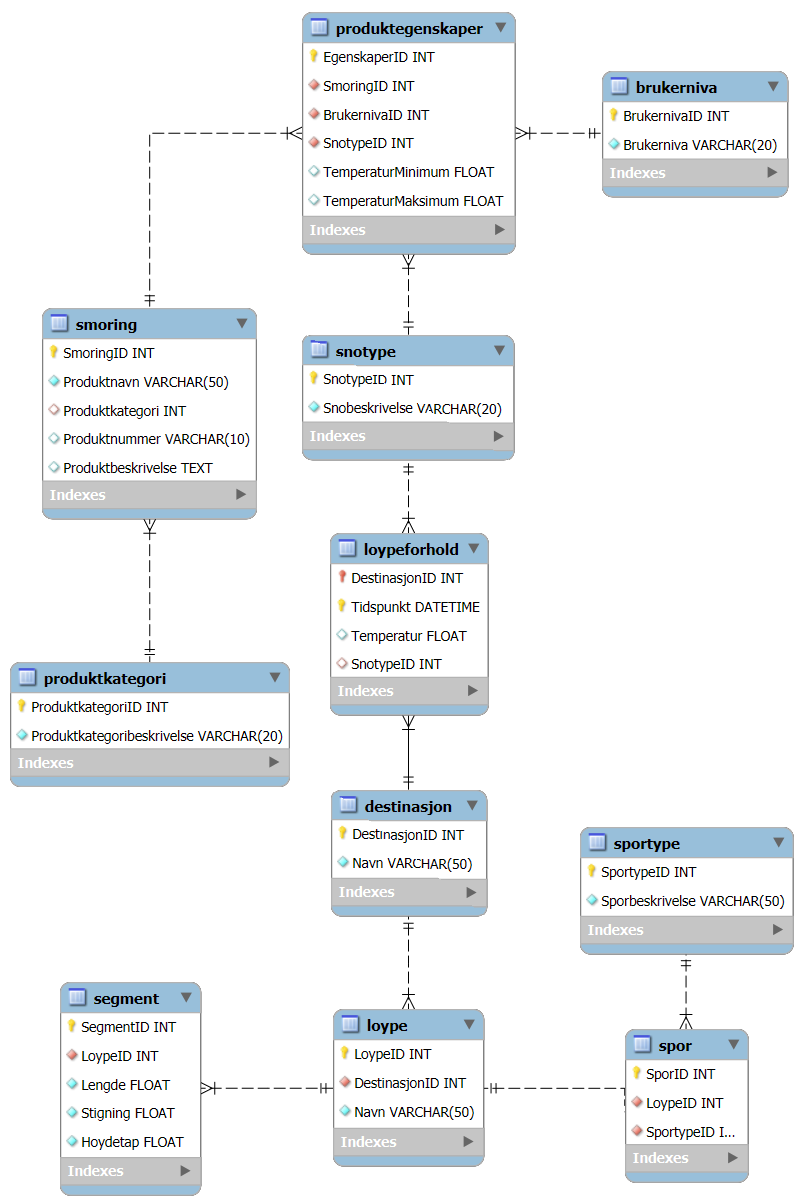
\includegraphics[width=\textwidth]{ermodell.png}

\section{Database implementasjon}

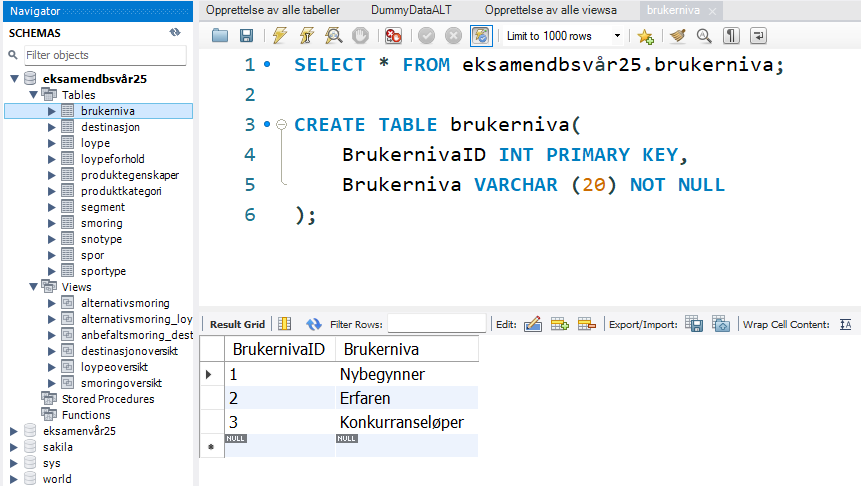
\includegraphics[width=\textwidth]{brukerniva.png}
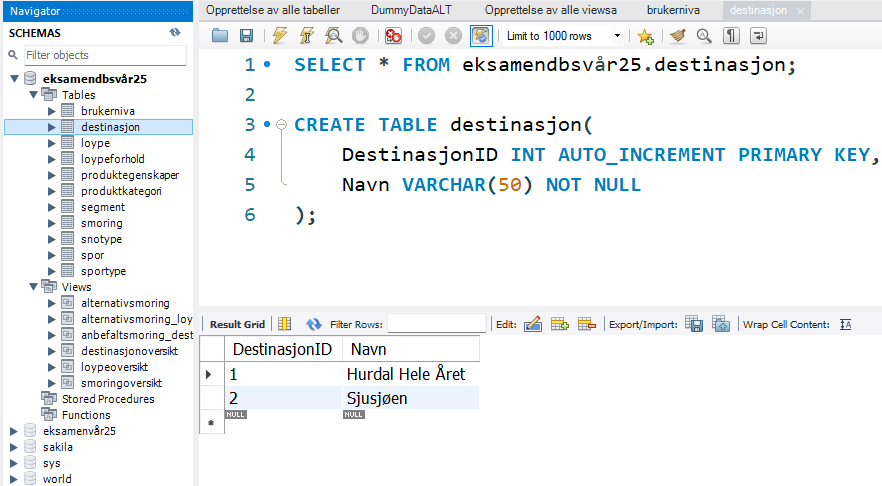
\includegraphics[width=\textwidth]{destinasjon.png}
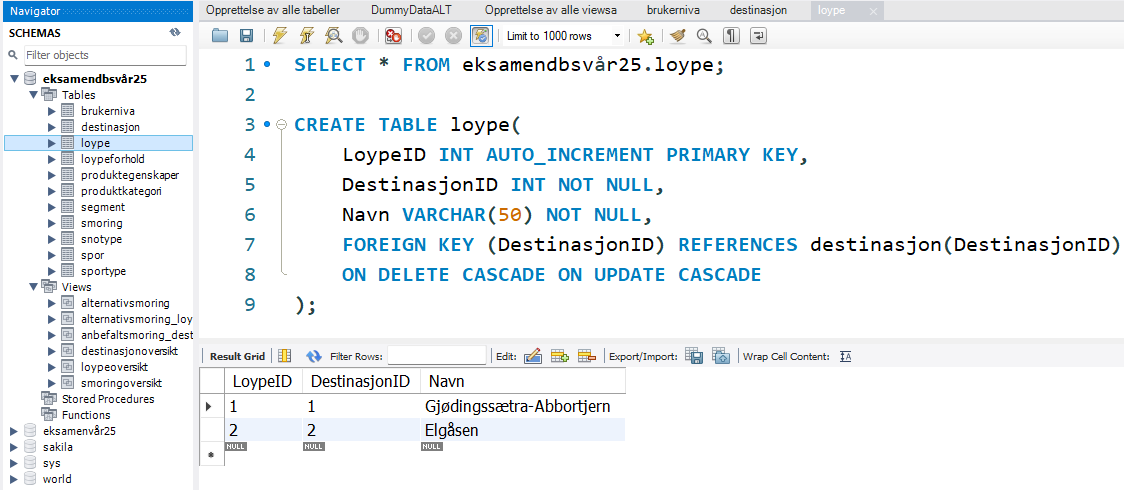
\includegraphics[width=\textwidth]{loype.png}
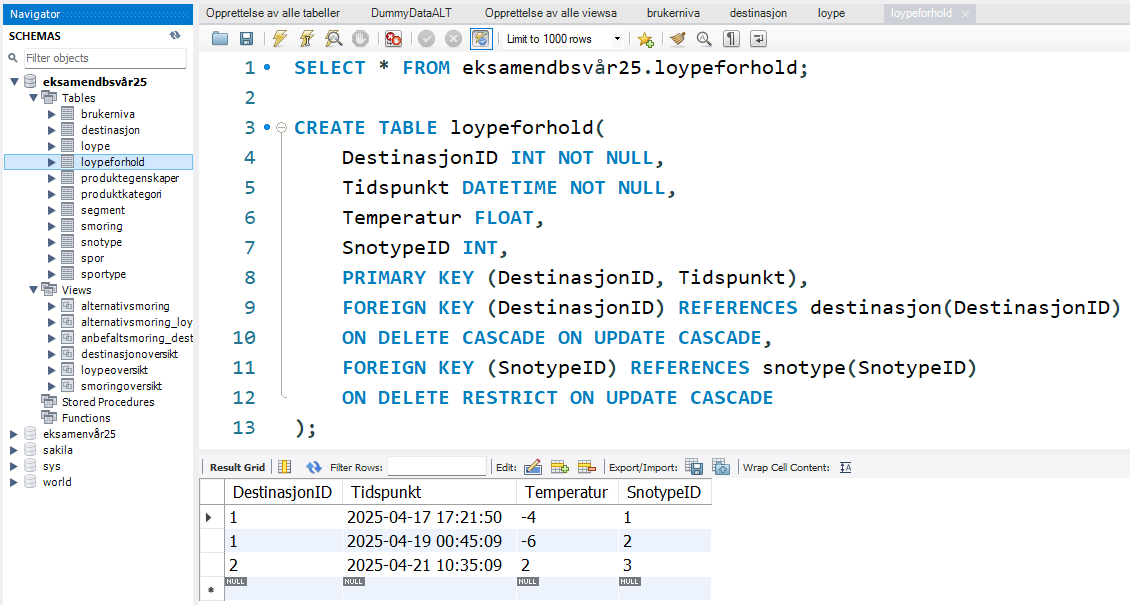
\includegraphics[width=\textwidth]{loypeforhold.png}
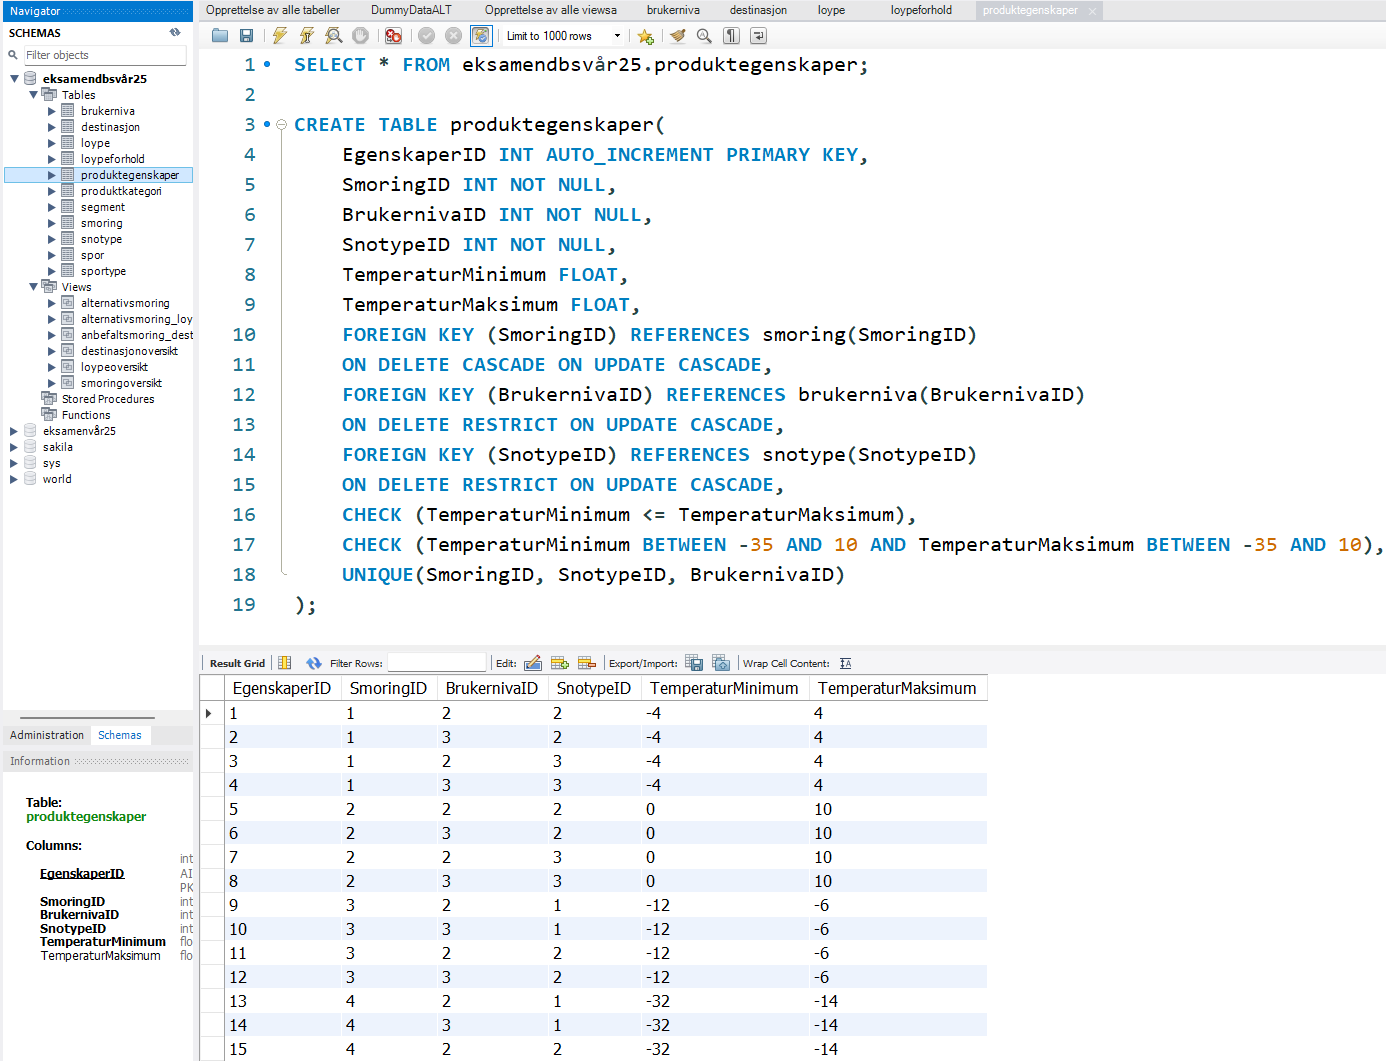
\includegraphics[width=\textwidth]{produktegenskaper.png}
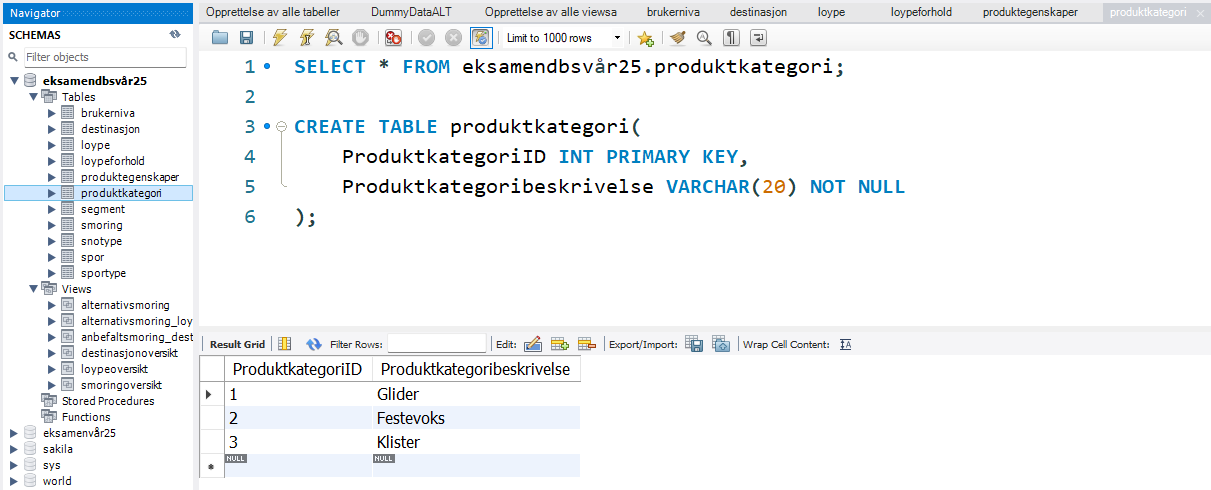
\includegraphics[width=\textwidth]{produktkategori.png}
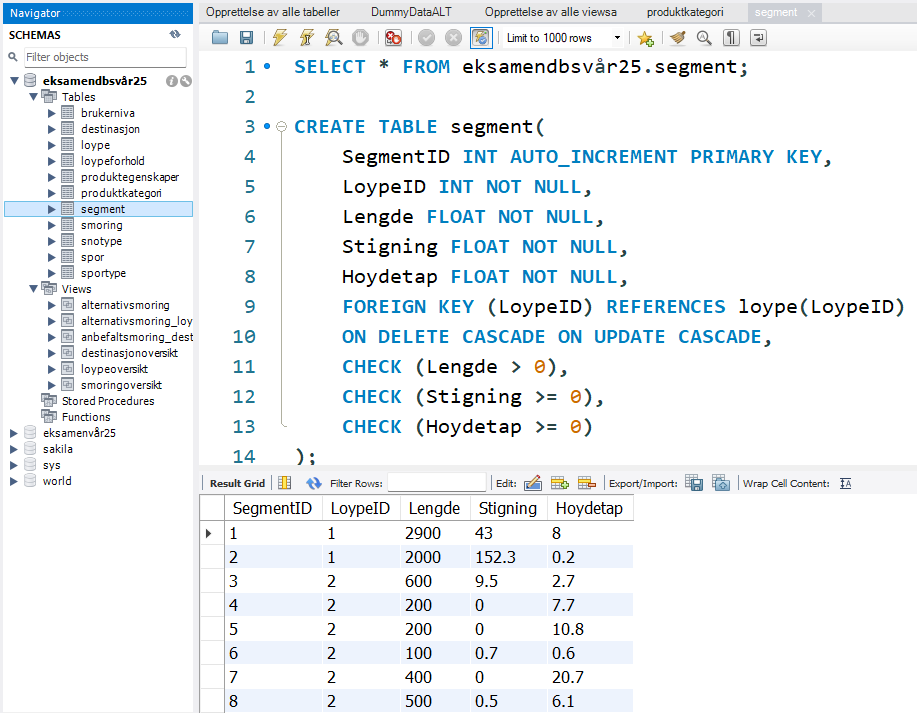
\includegraphics[width=\textwidth]{segment.png}
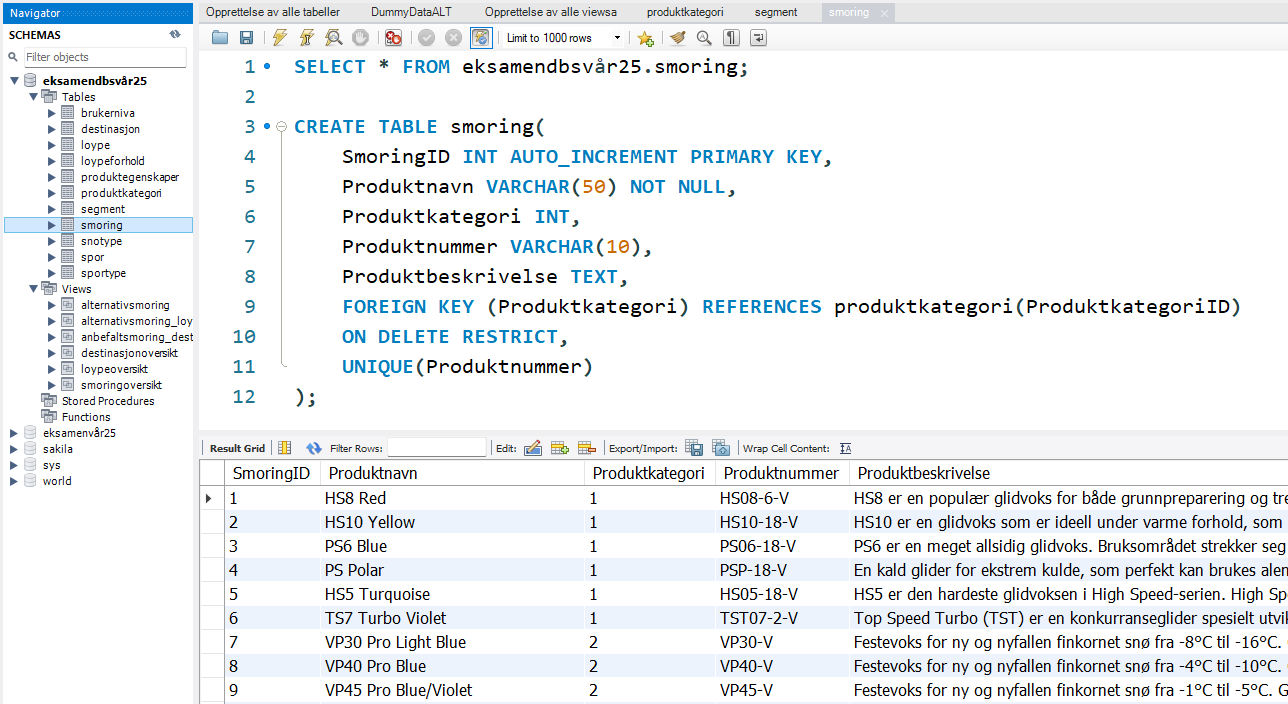
\includegraphics[width=\textwidth]{smoring.png}
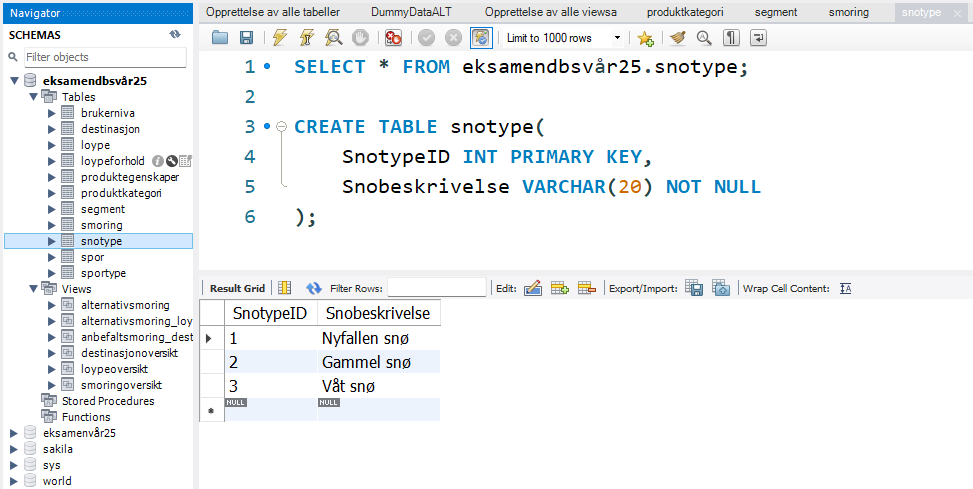
\includegraphics[width=\textwidth]{snotype.png}
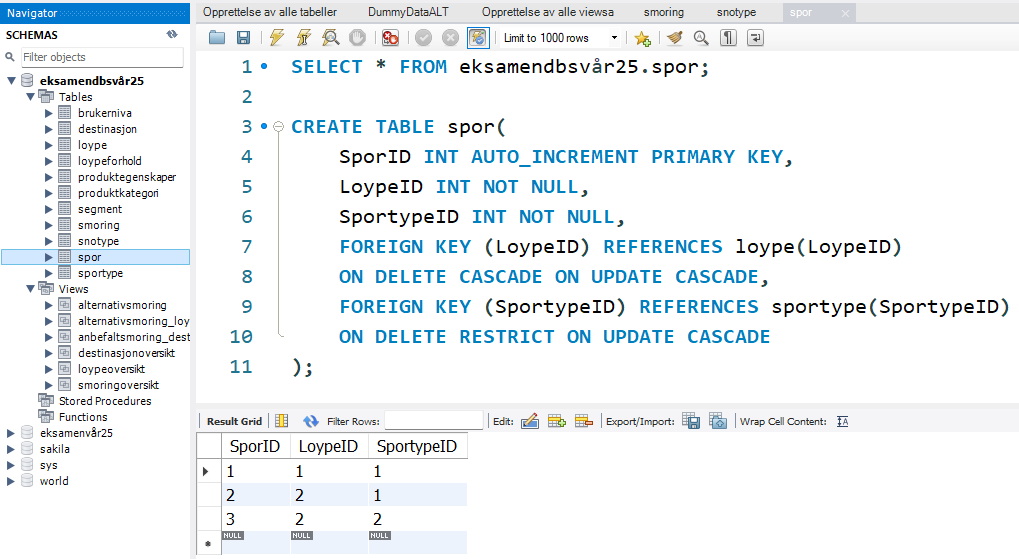
\includegraphics[width=\textwidth]{spor.png}
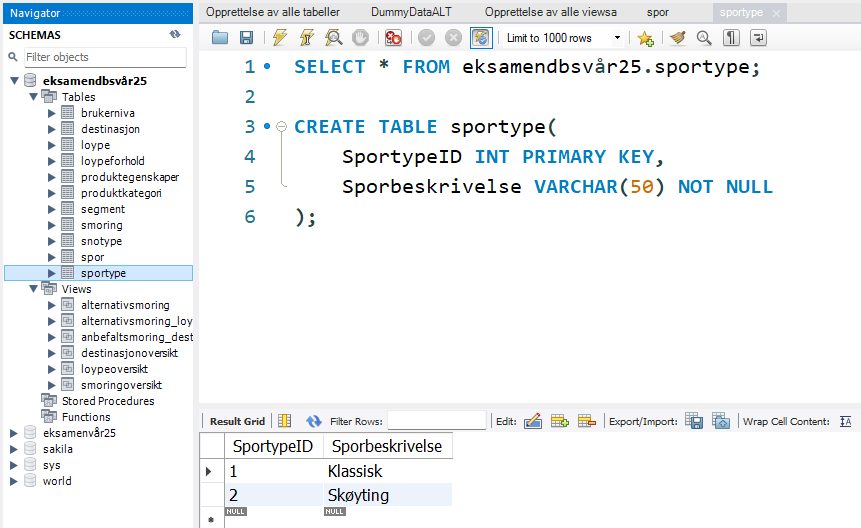
\includegraphics[width=\textwidth]{sportype.png}

\section{Dummy data}

Hovedformål med dummydata:
Forklare hvorfor dummydata er nødvendig og hva vi tenker at den skal demonstrere. Altså systemets funksjonelle krav og generelle spesifikasjoner. Vi har derfor valgt å ta med realistiske eksempler på ... smøring, løyper, løypeforhold og brukernivå. 

Hvordan har vi tenkt?:
Forklare hvilke tabeller vi har fylt med dummydata og hva tanken bak tabellen er. Hvilke varianter har vi med av smøringer? Produktkategorier, Temperaturintervall osv...

Begrunnelse:
Her forklarer vi hvorfor nettopp dataen vi har brukt ble valgt og forklarer at de dekker et bredt spekter av skismøring med ulike kombinasjoner. Alle smøringer er realistiske fra Swix sine produkter og det sørger videre for at alle views og spørringer gir meningsfulle resultater

\section{SQL-spørringer}

Navn på spørringen: Anbefaltsmøringalternativ f.eks

Hvilket systemkrav prøver vi å oppfylle med denne spørringen - hva skal spørringen gjøre?: Forklarer da hvilket resultat spørringen fører til og hvilket systemkrav den oppfyller.

Kommentere SQL-spørringen: Her kommenter vi SQL-koden under hver linje og forklarer nøyaktig hva som skjer

Eksempel på resultat: Her tar vi med skjermbilde av resultatet, f.eks to eller tre rader (hvis ikke bare ett resultat)

Begrunnelse: Forklarer her hvorfor spørringen er logisk og hvordan f.eks temperaturinput henger sammen med at den faller mellom et gitt temperaturintervall....

% section  (end)
\end{document}
